%%%%%%%%%%%%%%%%%%%%%%%%%%%%%%%%%%%%%%%%%
% Developer CV
% LaTeX Template
% Version 1.1 (February 24, 2025)
%
% This template originates from:
% https://www.LaTeXTemplates.com
%
% Authors:
% Jan Vorisek (jan@vorisek.me)
% Based on a template by Jan Küster (info@jankuester.com)
% Modified for LaTeX Templates by Vel (vel@LaTeXTemplates.com)
%
% License:
% The MIT License (see included LICENSE file)
%
%%%%%%%%%%%%%%%%%%%%%%%%%%%%%%%%%%%%%%%%%

%----------------------------------------------------------------------------------------
%	PACKAGES AND OTHER DOCUMENT CONFIGURATIONS
%----------------------------------------------------------------------------------------

\documentclass[10pt]{../developercv} % Default font size, values from 8-12pt are recommended
\usepackage{graphicx}
\graphicspath{{../images/}} % Path to the images folder

%----------------------------------------------------------------------------------------

\begin{document}

%----------------------------------------------------------------------------------------
%	TITLE AND CONTACT INFORMATION
%----------------------------------------------------------------------------------------

\begin{minipage}[t]{0.47\textwidth} % Left column with your name and title, change the width as needed
	\vspace{-\baselineskip} % Required for vertically aligning minipages

	% If your name is very short: use just one of the lines below
	% If your name is very long: reduce the font size or make the current column wider (and reduce the others proportionately)
	\colorbox{black}{{\HUGE\textcolor{white}{\textbf{\MakeUppercase{Stefan}}}}} % First name

	\colorbox{black}{{\HUGE\textcolor{white}{\textbf{\MakeUppercase{Schärmeli}}}}} % Last name

	\vspace{6pt} % Vertical whitespace

	{\LARGE Fullstack DevOps Engineer} % Career or current job title
\end{minipage}
\hfill % Automatic horizontal whitespace
\begin{minipage}[t]{0.25\textwidth} % Center column with the first column of icons
	\vspace{-\baselineskip} % Required for vertically aligning minipages

	% The first parameter is the FontAwesome icon name, the second is the box size and the third is the text
	% Other icons can be found by referring to fontawesome5.pdf (supplied with the template) and using the word after \fa in the command for the icon you want
	\icon{MapMarker}{12}{Bern}\\
	\icon{BirthdayCake}{12}{02.06.1983}\\
	\icon{Ring}{12}{ledig}\\
	\icon{Phone}{12}{+41 76 368 66 16}
\end{minipage}
\hfill % Automatic horizontal whitespace
\begin{minipage}[t]{0.23\textwidth} % Center column with the first column of icons
	\vspace{-\baselineskip} % Required for vertically aligning minipages
	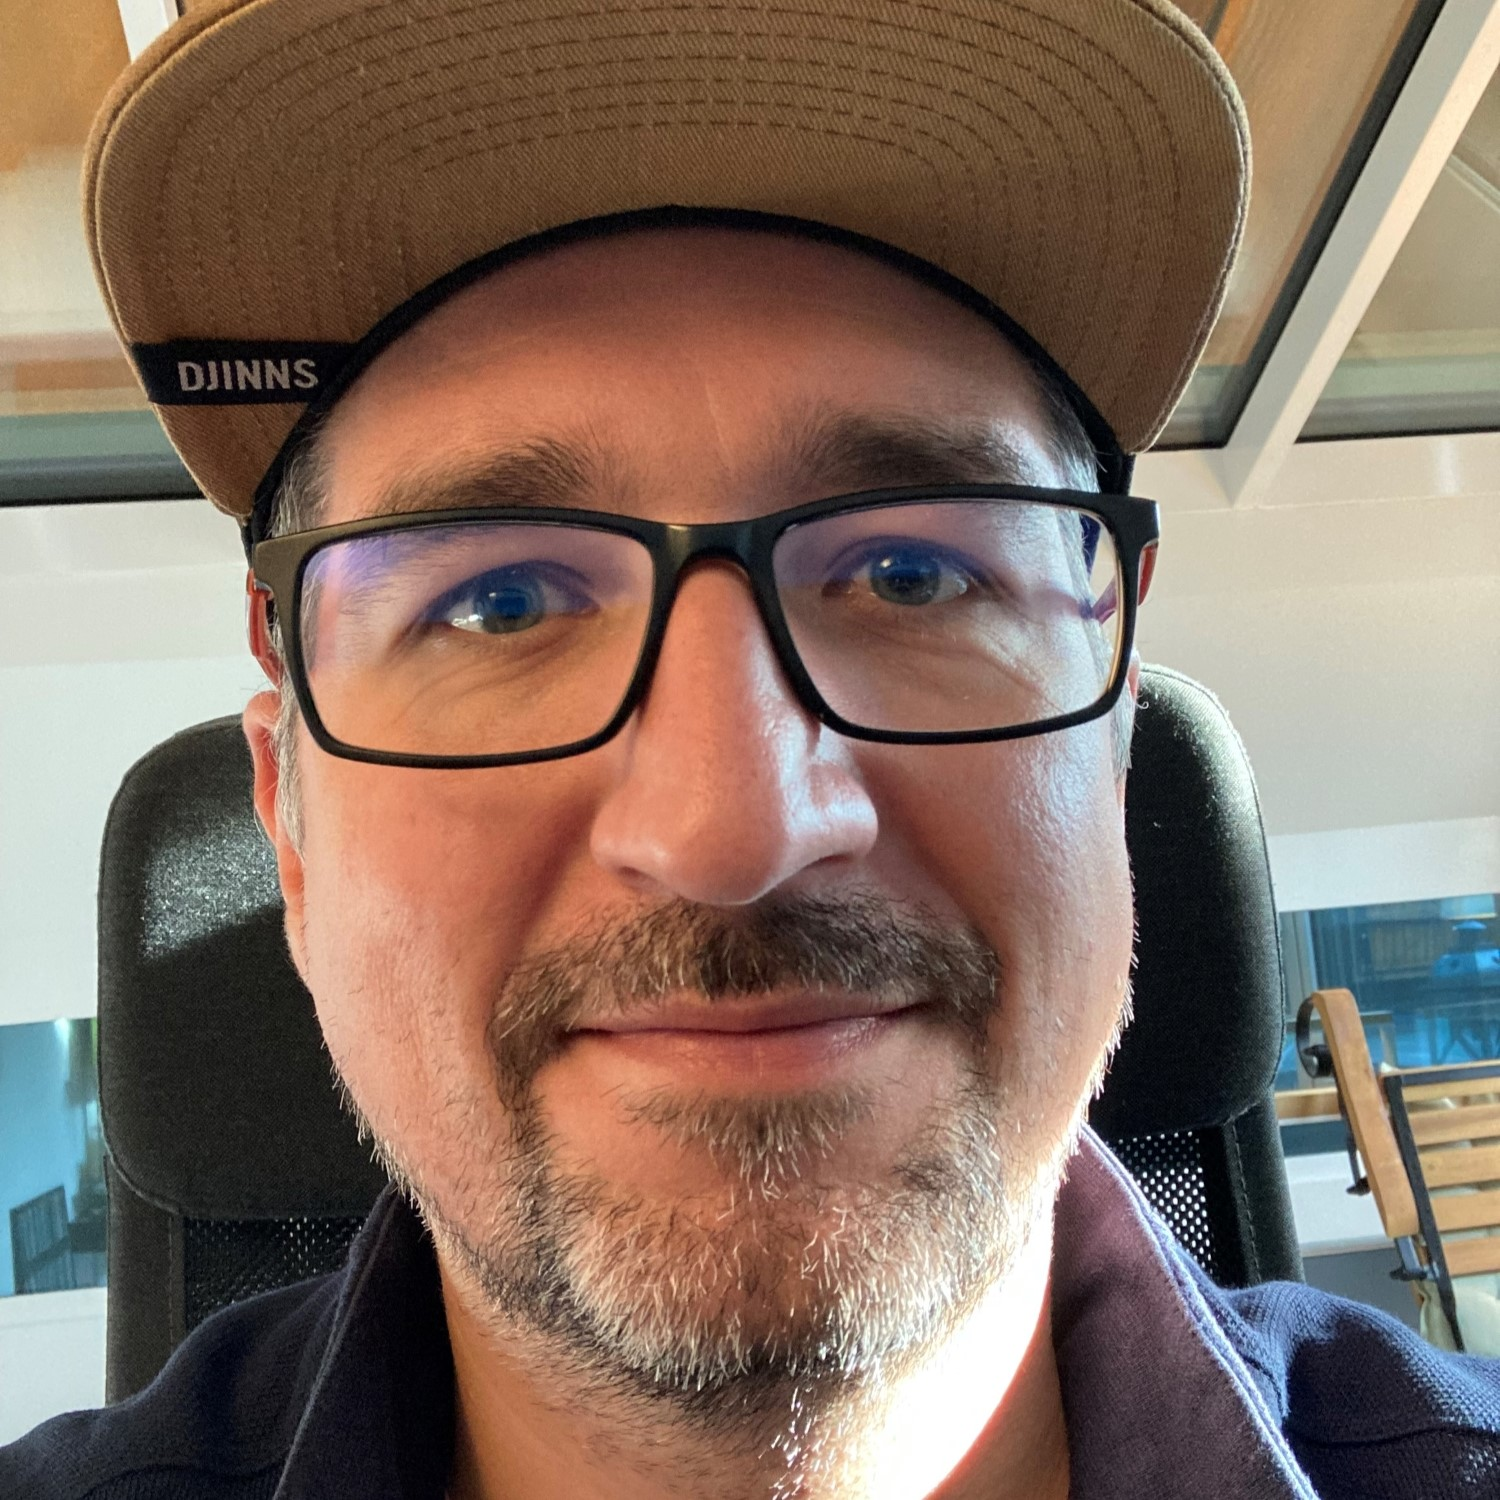
\includegraphics[width=0.8\textwidth]{schaermu_quad.jpg}
\end{minipage}
\hfill % Automatic horizontal whitespace

\vspace{0.75cm} % Vertical whitespace

\begin{minipage}[t]{1\textwidth} % Center column with the first column of icons
	\vspace{-\baselineskip} % Required for vertically aligning minipages

	% The first parameter is the FontAwesome icon name, the second is the box size and the third is the text
	% Other icons can be found by referring to fontawesome5.pdf (supplied with the template) and using the word after \fa in the command for the icon you want
	\icon{At}{12}schaermu@pm.me\hspace{0.2cm}
	\icon{Globe}{12}schaermu.ch/cv\hspace{0.2cm}
	\icon{Github}{12}github.com/schaermu\hspace{0.2cm}
\end{minipage}

\vspace{0.5cm} % Vertical whitespace

%----------------------------------------------------------------------------------------
%	INTRODUCTION, SKILLS AND TECHNOLOGIES
%----------------------------------------------------------------------------------------

\cvsect{Wer bin ich?}

\begin{minipage}[t]{0.4\textwidth} % Left column with the introduction text, change the width as needed
	\vspace{-\baselineskip} % Required for vertically aligning minipages
	Seit ich in den 90ern die ersten BASIC-Scripts aus dem AMIGA-Magazin minutiös in meinen Amiga 600 abgetippt habe, hat mich die Faszination Software-Entwicklung mit all ihren Facetten nicht mehr losgelassen. Die Aussage «Mach doch einfach dein Hobby zum Beruf» des Inhabers eines Grafikateliers setzte den Startschuss für eine abwechslungsreiche Laufbahn in der Informatik, für welche ich auch über 20 Jahre später immer noch brenne wie am ersten Tag.\\
\end{minipage}
\hfill % Automatic horizontal whitespace
\vspace{0.25cm} % Vertical whitespace
\begin{minipage}[t]{0.5\textwidth} % Right column with the skills bar chart, change the width as needed
	\vspace{-\baselineskip} % Required for vertically aligning minipages

	\begin{barchart}{5.5} % The parameter to the barchart environment is the maximum width (in cm) of the longest bar}
		\baritem{CI/CD}{90}
		\baritem{Git}{90}
		\baritem{Backend-Dev}{80}
		\baritem{Container}{70}
		\baritem{Linux/Shell}{60}
		\baritem{Cloud (AWS)}{60}
		\baritem{Monitoring}{40}
	\end{barchart}
\end{minipage}

% Output a series of bubbles showing your proficiency with environments and/or tools
\begin{center}
	\bubbles{4/GitLab, 5/GitHub, 4/Go, 6/VS Code, 5/Git, 5/TypeScript, 5/AWS, 4/Python} % Each bubble must be in the format of '<size>/<label>' and you can specify as many bubbles as will fit on the page
\end{center}

%----------------------------------------------------------------------------------------
%	EXPERIENCE
%----------------------------------------------------------------------------------------

\cvsect{Berufserfahrung}

\begin{entrylist}
	\entry
	{\footnotesize 10/2022 -- heute}
	{Requirements-to-Deployment Manager}
	{Post CH AG}
	{In der Rolle des Requirements-to-Deployment Manager verantworte ich die fachliche Führung im Bereich Software-Entwicklung von 13 Teams und unterstütze sie in allen Belangen der Software-Entwicklung als Coach und Mentor. Dies kann viele Bereiche betreffen, wie zum Beispiel Requirements Engineering, Way of Work, Methoden, Standard-Tools \& Developer Experience oder CI/CD \& Automation. Wo nötig, helfe ich den Teams auch in der Implementierung aus, beispielsweise bei Migrationen auf neue CI/CD-Plattformen, Adaption von neuen Vorgehensmodellen oder bei der Planung von technologischen Lifecycles.\\ \\
		In enger Zusammenarbeit mit dem Leitungsteam von IT12 treibe ich zusätzlich die strategische Weiterentwicklung der Unit voran. Dazu gehört die Etablierung diverser Werkzeuge zur Strategie-Umsetzung wie beispielsweise OKR, Portfolio-Management oder Reporting-Dashboards.\\ \\
		Als Cloud-Portfolio Owner bin ich auch für das  Vorantreiben des konzernweiten Post2Cloud-Vorhabens innerhalb unserer Abteilung verantwortlich und unterstütze die Teams bei der Planung und Umsetzung der Migration auf moderne Cloud-Technologien und -Plattformen.\\ \small \texttt{CI/CD}\slashsep\texttt{SAFe \& Scrum}\slashsep\texttt{Cloud}\slashsep\texttt{Way-of-Work}\slashsep\texttt{Strategie \& OKR}\slashsep\texttt{Leadership}}
	\entry
	{\footnotesize 11/2018 -- 10/2022}
	{Full-Stack-Entwickler}
	{Post CH AG}
	{In einem kleinen, schlagkräftigen Team durfte ich diverse Proof-of-Concepts und marktfähige MVPs für unsere Geschäftsbereiche mit verschidensten Web-, AR-, Voice- und KI-Technologien entwickeln. Dabei lag ein starker Fokus auf Design-Thinking Ansätzen mit den involvierten Stakeholdern um innert kürzester Zeit den maximalen Effekt zu erzielen und Ideen schnell am Markt testen zu können. Zusätzlich durfte ich beim Aufbau einer internen, cloud-basierten Betriebsplattform für Innovations-Vorhaben sowie in diversen internen Innovations-Vorhaben und -Arbeitsgruppen aktiv sein.\\ \\Von 2020 bis 2022 war ich als Co-Lead für die Entwicklung und den Rollout eines Security-Champion Programms innerhalb der IT-Entwicklung mitverantwortlich.\\ \small \texttt{Prototyping}\slashsep\texttt{Security}\slashsep\texttt{Terraform}\slashsep\texttt{dotnet Core}\slashsep\texttt{Postgres}\slashsep\texttt{Angular}\slashsep\texttt{Cloud-Engineering}}
	\entry
	{\footnotesize 10/2016 -- 10/2018}
	{Full-Stack-Entwickler}
	{smartfactory GmbH}
	{In einem kleinen, multi-nationalen Team bestehend aus App- und Backend-Entwicklern durfte ich die Umsetzung diverser Kundenprojekte begleiten. Diese wurden mehrheitlich in Django (Python-Framework) sowie Vue.js- oder Ionic-basierenden Frontends umgesetzt.\\ \\ Neben dem Projektgeschäft habe ich die Modernisierung der CI/CD-Plattform auf GitLab sowie die Automatisierung aller Release- und Deploymentprozesse mit Ansible aktiv vorangetrieben und implementiert.\\ \small \texttt{Django}\slashsep\texttt{Laravel}\slashsep\texttt{Angular}\slashsep\texttt{Linux}\slashsep\texttt{Ansible}\slashsep\texttt{CI/CD}}

	\entry
	{\footnotesize 06/2012 -- 05/2016}
	{Software-Entwickler / Teamleiter}
	{Maxomedia AG}
	{Als Mitglied eines Software-Teams begleitete ich die agile Umsetzung diverser Kundenprojekte gemeinsam mit Vertretern aus der Kreativ-Abteilung der Agentur, unter anderem nationale Kampagnen für die SBB, Postfinance oder Postauto. Auch hier habe ich stark an der Modernisierung der CI/CD-Pipeline sowie agilen Arbeitsmethoden mitgewirkt. Ab Anfang 2015 durfte ich die Teamleitung für ein Team von 4 Entwicklern sowie die technische Verantwortung für die interne CI/CD-Infrastruktur und -Prozesse übernehmen.\\ \small \texttt{Dotnet}\slashsep\texttt{node.js}\slashsep\texttt{MSSQL Server}\slashsep\texttt{CI/CD}\slashsep\texttt{Leadership}\slashsep\texttt{Scrum}}

	\entry
	{\footnotesize 10/2003 -- 05/2012}
	{Web-Entwickler}
	{diverse Firmen}
	{Während der Zeit nach der Ausbildung durfte ich in verschiedenen Firmen Individuallösungen für Kunden wie Kuoni, Migros, Hotelplan oder Banken implementieren und betreuen. Bei jeder dieser Stationen war das Thema CI/CD präsent, in unterschiedlichen Ausprägungen: teilweise ging es um einen Aufbau solcher Prozesse von Grund auf, in anderen Umfeldern ging es um eine Weiterentwicklung und Modernisierung. Technologisch bewegte ich mich grösstenteils in Dotnet, PHP und node.js in meiner Funktion als Web-Entwickler.\\ \small \texttt{Dotnet}\slashsep\texttt{PHP}\slashsep\texttt{node.js}\slashsep\texttt{Linux}\slashsep\texttt{Apache/IIS}\slashsep\texttt{Server-Betrieb}\slashsep\texttt{CI/CD}}

\end{entrylist}

%----------------------------------------------------------------------------------------
%	EDUCATION
%----------------------------------------------------------------------------------------

\vspace{0.5cm} % Vertical whitespace
\cvsect{Ausbildung}

\begin{entrylist}
	\entry
	{\footnotesize 08/1999 -- 09/2003}
	{Ausbildung Informatiker EFZ}
	{SBB CH AG}
	{Ausbildung zum Informatiker EFZ bei der SBB CH AG (ab 2002 bei der login Berufsbildung AG) in der Fachrichtung Softwareentwicklung. Die Abschlussarbeit habe ich im Bereich Webentwicklung in PHP durchgeführt.}
\end{entrylist}

%----------------------------------------------------------------------------------------
%	ADDITIONAL INFORMATION
%----------------------------------------------------------------------------------------

\vspace{0.5cm} % Vertical whitespace
\begin{minipage}[t]{0.45\textwidth} % Left column width
	\vspace{-\baselineskip} % Required for vertically aligning minipages

	\cvsect{Sprachen}

	\textbf{Deutsch} -- Muttersprache\\
	\textbf{Englisch} -- C1\\
	\textbf{Französisch} -- A1/A2
\end{minipage}
\hfill % Automatic horizontal whitespace
\begin{minipage}[t]{0.45\textwidth} % Center column width
	\vspace{-\baselineskip} % Required for vertically aligning minipages

	\cvsect{Referenzen}

	auf Anfrage
\end{minipage}

%----------------------------------------------------------------------------------------

\end{document}
